%!TEX root = ../documentation.tex
\chapter{Datenanalyse}
\label{ch:data_analysis}

\section{Bilddaten}
\newlength{\imagewidth}

Wir betrachten zunächst die Bilddaten aus dem Datenset und stellen anhand von geeigneten Beispielen und Analysen heterogene Eigenschaften dieser dar, welche sich für das Training als problematisch erweisen könnten.

\begin{figure}[ht]
	\centering
	\begin{subfigure}[b]{0.45\textwidth}
		\includegraphics[width=\textwidth]{../images/34308.jpeg}
		\caption{34308.jpeg\\Originalgröße 1524 x 1516 Pixel}
	\end{subfigure} \hfill
	\begin{subfigure}[b]{0.45\textwidth}
		\includegraphics[width=\textwidth]{../images/65415.jpg}
		\caption{65415.jpg\\Originalgröße 369 x 320 Pixel}
	\end{subfigure}
	\caption{Zwei Bilder männlicher Patienten aus dem Datenset}
\end{figure}

Die Beispiele (a) und (b) lassen einen deutlich unterschiedlichen Kontrast erkennen. Bei Beispiel (a) handelt es sich zudem um ein Farbbild während es sich bei Beispiel (b) um ein Schwarzweißbild handelt. Die beiden Bilder weisen unterschiedliche Dimensionen auf.\\
Diese heterogenen Eigenschaften zeigen Komplexität innerhalb des Datensets, welche von einem gelernten Model entsprechend wiedergespiegelt werden müsste. Es ist also angebracht die Daten mittels geeigneter Vorverarbeitung zu homogenisieren.

Insgesamt werden die Unterschiede in Dimension und Farbe von den folgenden Grafiken dargestellt.

\begin{figure}[H]
	\centering
	\settowidth{\imagewidth}{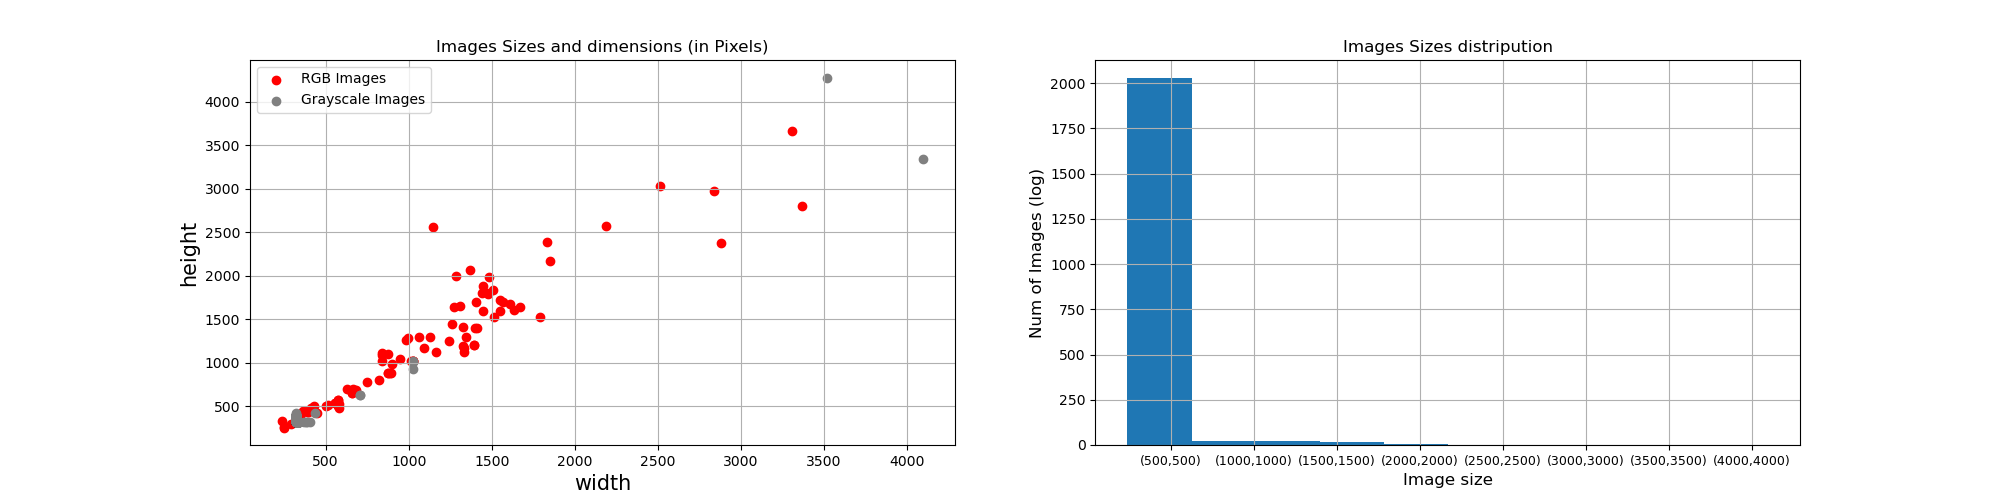
\includegraphics{../image_sizes.png}}
	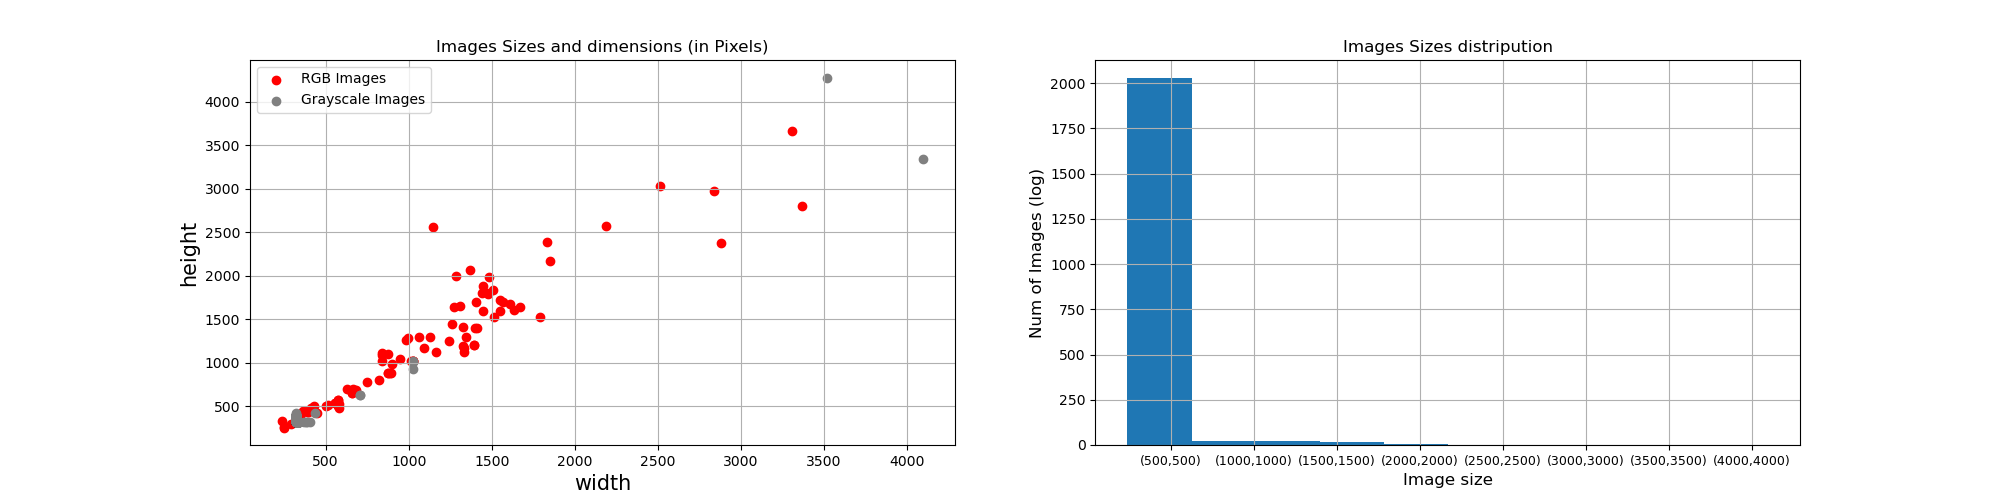
\includegraphics[trim=110px 0 0.5\imagewidth{} 0, clip,width=0.9\textwidth]{../image_sizes.png}
	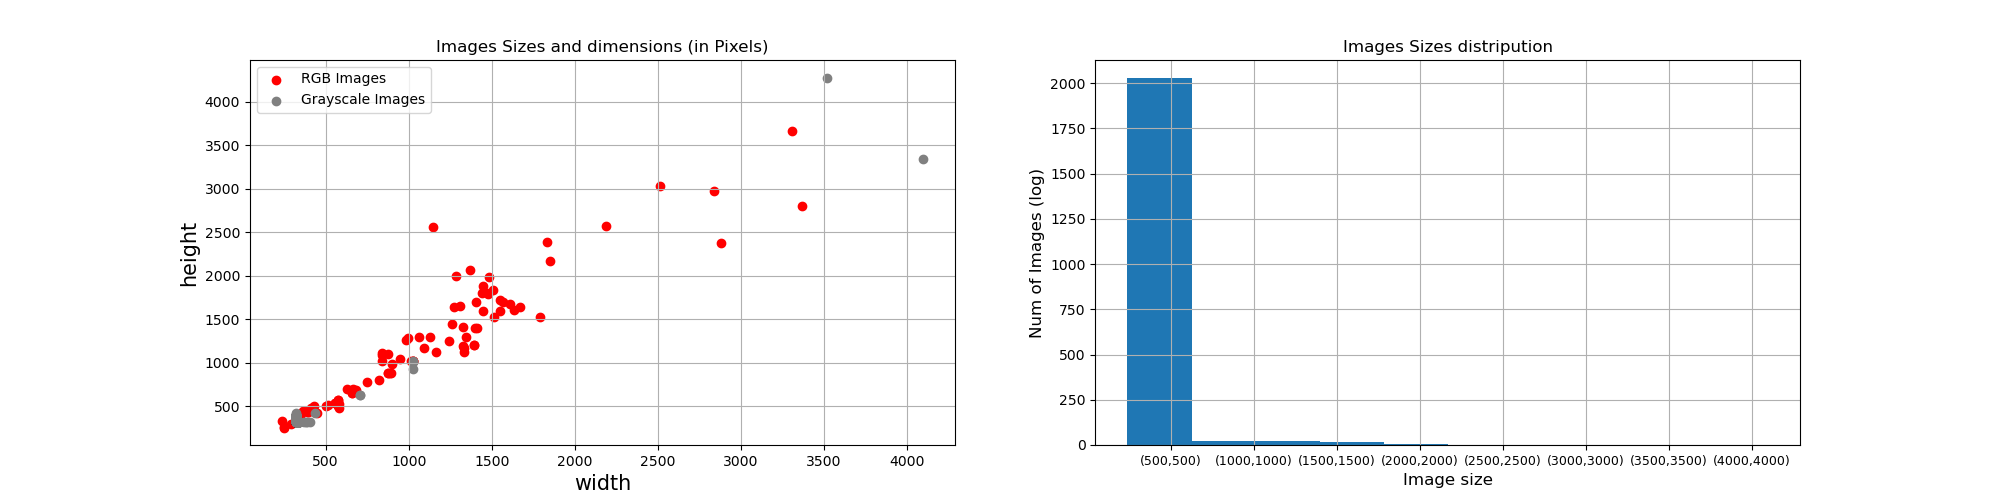
\includegraphics[trim=0.5\imagewidth{} 0 110px 0, clip,width=0.9\textwidth]{../image_sizes.png}
	\caption{Verteilung der Bilddimensionen}
\end{figure}

Von den Bildern sind 92 Farbbilder und 2008 Schwarzweißbilder. Ein Großteil der Dimensionen ist im Bereich von etwa 320 x 320 Pixeln angeordnet.

\section{Klassen}

Wir betrachten zunächst die Verteilung der drei Klassen (COVID-19 Erkrankung, Andere Erkrankung, Gesund) über das Datenset.

\begin{figure}[H]
	\centering
	\settowidth{\imagewidth}{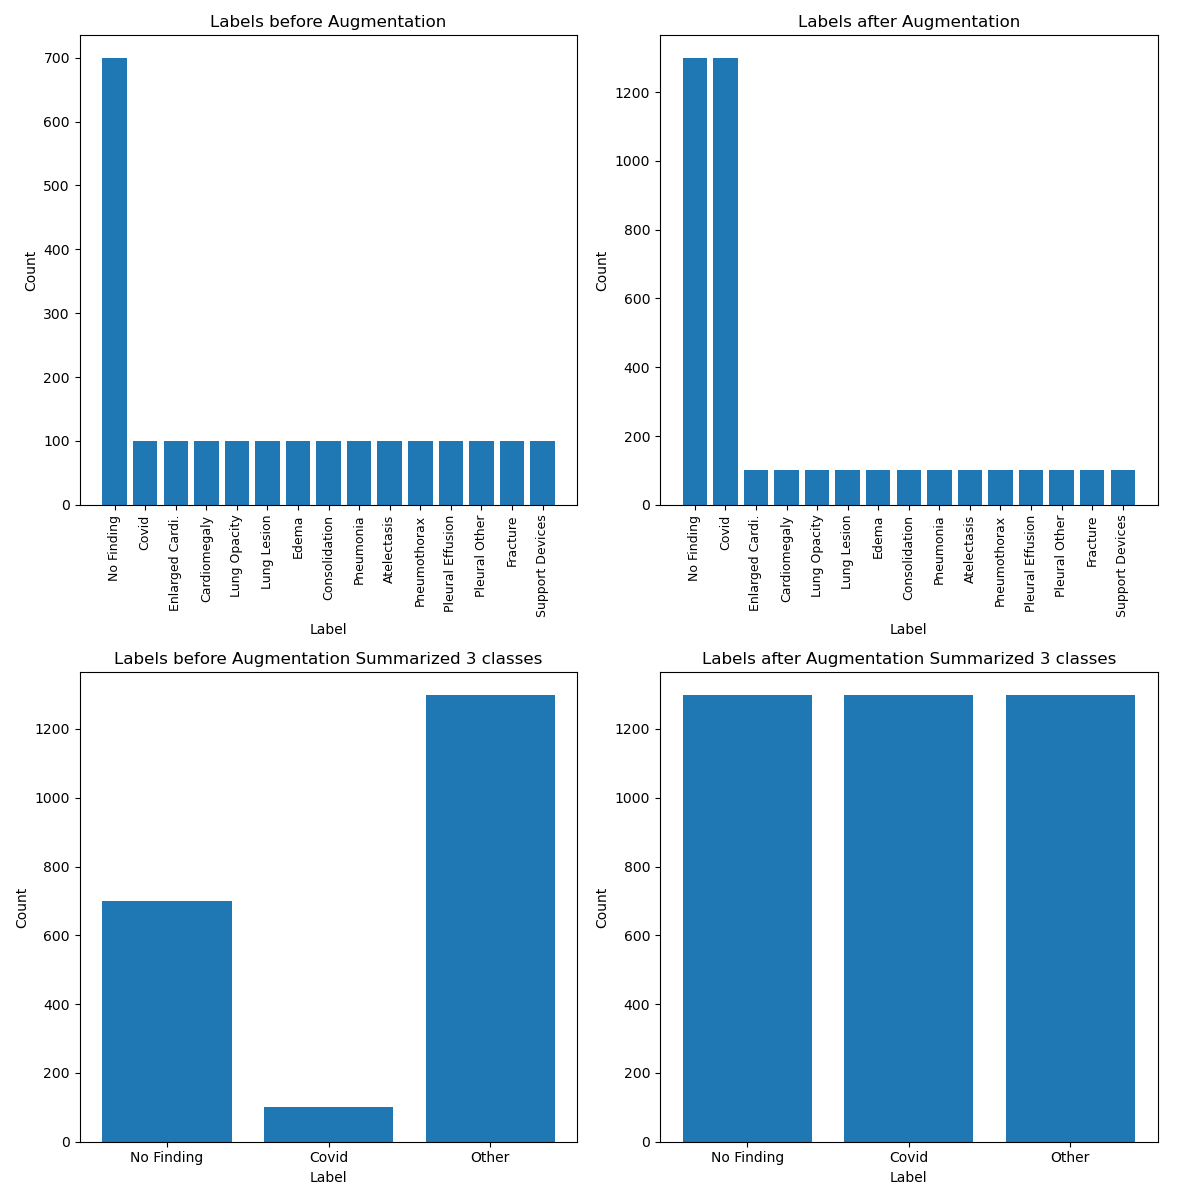
\includegraphics{../balancing.png}}
	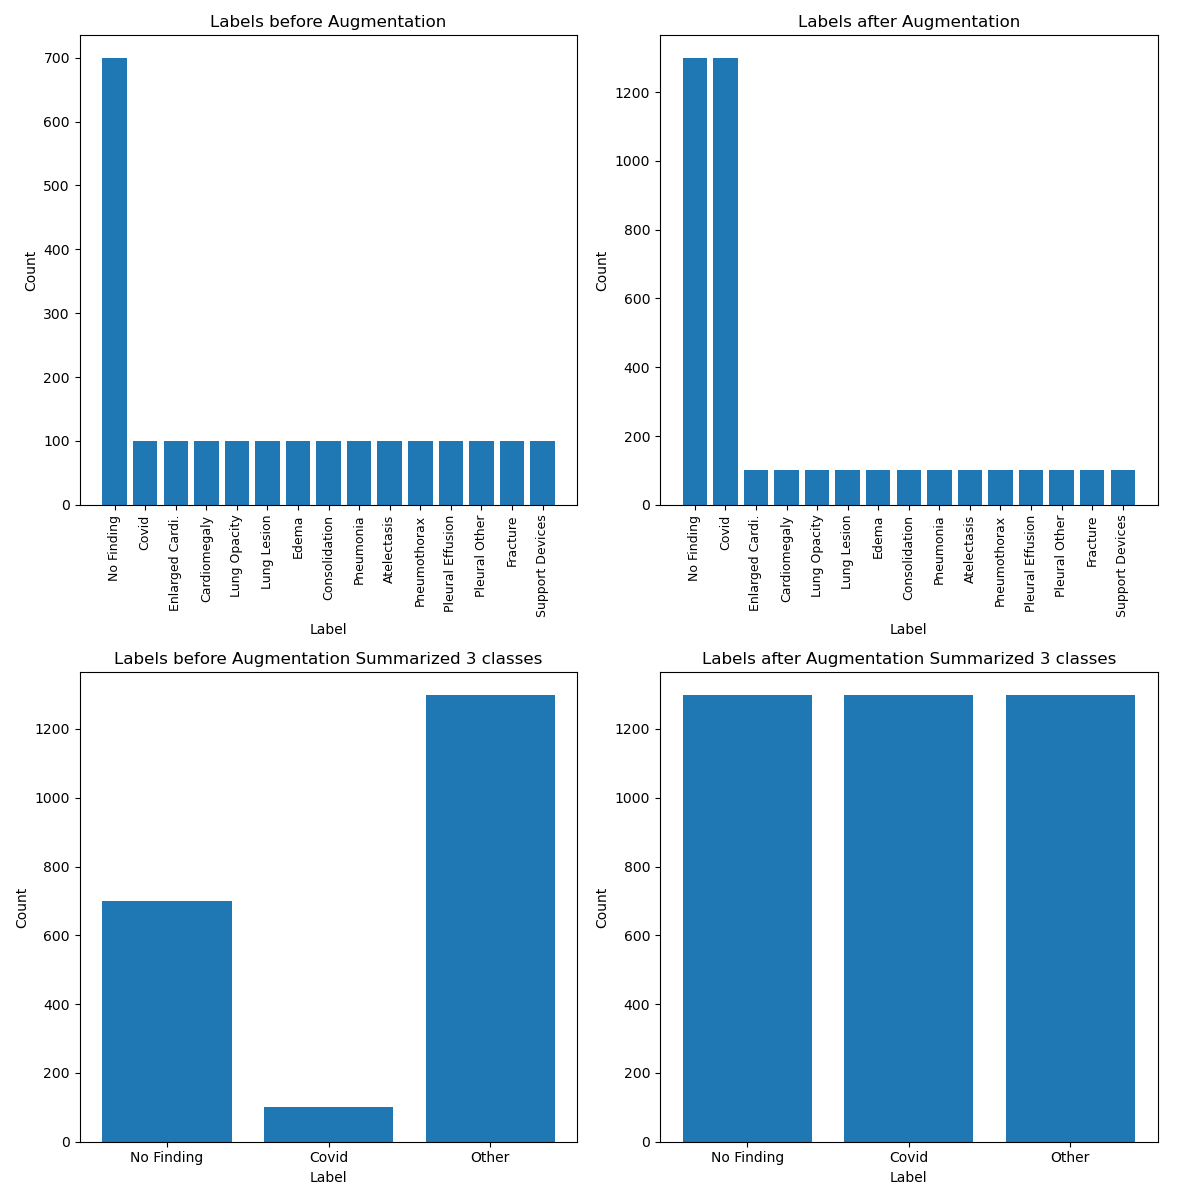
\includegraphics[trim=0 0 0.5\imagewidth{} 0, clip,width=0.3\imagewidth{}]{../balancing.png}
	\caption{Verteilung der Klassen}
\end{figure}

Der Anteil an COVID-19 Erkrankungen ist im Vergleich zu den anderen Klassen relativ gering.\\
Um eine gute Generalisierungsfähigkeit sicherzustellen, ist es sinnvoll zusätzliche Trainingsbeispiele aus der COVID-19 Klasse bereitzustellen.

Wir betrachten ebenfalls die Verteilung der Features Alter und Geschlecht innerhalb der COVID-19 Erkrankungen aus dem Datenset.

\begin{figure}[ht]
	\centering
	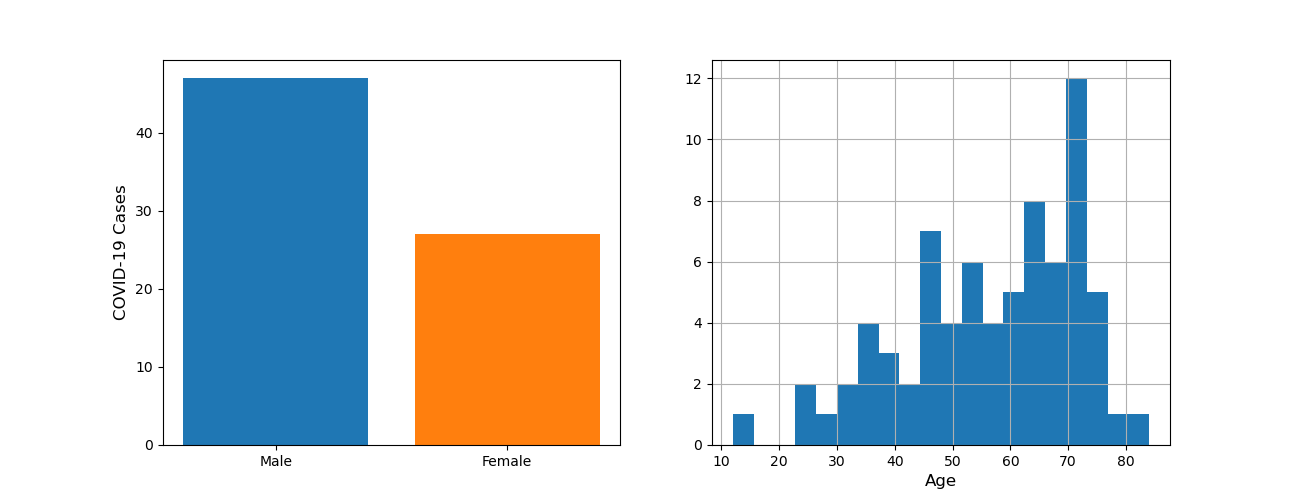
\includegraphics[width=\textwidth]{../features_analysis.png}
	\caption{Analyse der Features Alter und Geschlecht bei COVID-19 erkrankten Patienten}
\end{figure}

Die Anteile von männlichen Patienten ist höher als der von weiblichen. Ebenfalls sind Daten von eher älteren Patienten vorhanden. Das Durchschnittsalter beträgt 56,46 Jahre.\\
Eventuell sind weitere Maßnahmen zur Entzerrung der Daten sinnvoll.